\documentclass{amsart}

\input{../preamble_general.tex}

\author{Jalen Chrysos}
\title{Hall's Theorem}

\begin{document}
	\maketitle 
	
	Recall that a graph $G$ is \textit{bipartite} if it can be divided into two sets of vertices $V_1,V_2$ such that for every edge of $G$, one vertex is in $V_1$ and the other is in $V_2$. 
	
	\begin{figure}[h]
		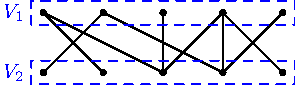
\includegraphics[width=6cm]{./Asymptote_Figs/Bipartite.pdf}
	\end{figure}
	
	\noindent A \textit{perfect matching} of $G$ is a collection of edges in $G$ that includes every vertex exactly once.
	
	\begin{figure}[h]
		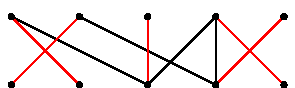
\includegraphics[width=6cm]{./Asymptote_Figs/Bipartite2.pdf}
	\end{figure}
	
	\noindent \underline{\textbf{Question}}: Given a bipartite graph $G$, how can we determine whether $G$ has a perfect matching?\\
	
	Hall's theorem answers this. Before stating the theorem, let's look at an example: \\
	
	\noindent \textbf{Example 1}: Does the following bipartite graph admit a perfect matching?
		
	\begin{figure}[h]
		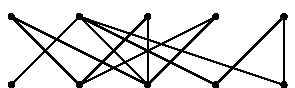
\includegraphics[width=6cm]{./Asymptote_Figs/Bipartite3.pdf}
	\end{figure}
	
	\textbf{Solution}: No. Observe the following induced subgraph:
		
	\begin{figure}[h]
		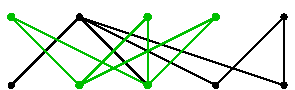
\includegraphics[width=6cm]{./Asymptote_Figs/Bipartite4.pdf}
	\end{figure}
	
	The three vertices in the upper part of the induced subgraph can only be matched to the two vertices in the lower part, but this means that multiple edges will include the same vertex in the lower part, by Pigeonhole principle. Thus, there can be no perfect matching.\\
	
	From this example, we make the observation that if any subset $A\subseteq V_1$ or $A\subseteq V_2$ has $|N(A)|<|A|$ (where $N(A)$ is the set of neighbors of vertices in $A$), then there can be no perfect matching. Hall's theorem tells us that the converse is also true:\\
	
	\noindent \textbf{Theorem (Hall)}: A bipartite graph $G$ has a perfect matching iff for all $A\subseteq V_1$ and $A\subseteq V_2$, $|N(A)|\geq |A|$.\\
	
%	In generalization,\\
%	
%	\noindent \textbf{Theorem (Tutte)}: Any graph $G$ has a perfect matching iff for all $A\subseteq G$, $G-A$ (the subgraph induced by removing $A$) has at most $|A|$ connected components with an \textit{odd} number of vertices.\\
	
%	\begin{proof}
%		This can be done by induction on the number of vertices in each part of $G$. If each part has $1$ vertex, the statement is just saying that one edge exists, which is a perfect matching on its own.\\
%		
%		Now suppose that Hall's theorem is true for graphs whose parts have size at most $n$. Let $G$ have two parts of $n+1$ vertices each, and suppose that $|N(A)|\geq |A|$ for all $A\subseteq V_1$ and $A\subseteq V_2$. We would like to choose two vertices $v\in V_1$ and $w\in V_2$ connected by an edge such that if the edge $v\sim w$ is \textit{removed}, we can find a perfect matching among the other vertices via the inductive hypothesis. But we need to ensure that removing $v$ and $w$ does not disrupt the $|N(A)|\geq |A|$ condition, i.e. that there is no $A\subset V_1\setminus \{v\}$ such that $w\in N(A)$ and $|N(A)|=|A|$. 
%		
%		Suppose for the sake of contradiction that for some $v$, every $w\in N(v)$ had the property that for some $A_w\subseteq V_1 \setminus \{v\}$, $|N(A_w)|=|A_w|$. Then letting $A = \cup_{w\in N(v)} A_w$, we see that 
%		$$N(A) = \bigcup_{w\in N(v)} N(A_w) \;\;\; \textbf{not done}\;\;\;|N(A)| \leq |A|$$
%		but then because $N(A\cup \{v\}) = N(A)$,  $|N(A\cup \{v\})|=|A| < |A\cup \{v\}|$, contradicting the premise.
%		
%	\end{proof}\\
	
	\newpage
	
	\bigskip
	
	\noindent \textbf{Problem 1}: Show that if $G$ is bipartite and all of its vertices have the same, nonzero degree, then $G$ has a perfect matching.\\
	
	\noindent \textbf{Problem 2}: Suppose that a standard deck of 52 cards is dealt into 13 piles of 4 cards each. Show that we can remove one card from each pile such that all the removed cards have different rank. Can we do the same with the remaining three-card piles?\\
	
	\noindent \textbf{Problem 3}: Two sheets of square paper are each subdivided into $n$ regions of area 1, and laid on top of one another. Show that there is a way to stick $n$ needles through the two papers such that every region in both papers is pierced by exactly one needle. Is this still possible if we have 3 sheets of paper instead of 2?\\
	
	\noindent \textbf{Problem 4} ($\star$): In a certain puzzle, an $n\times n$ grid is filled with the numbers $1,\dots,n^2$ in some order, and you are asked to put the numbers in order. To do this, you can use two types of moves: you can permute the elements within each row without moving any element out of its row, or you can permute the elements within the columns without moving any element out of its column. In the worst case, how many moves will it take you to solve this puzzle?
	
	$$
	\begin{bmatrix}
		1 & 4 & 7 & 13\\
		3 & 5 & 8 & 11 \\
		2 & 10 & 14 & 16\\
		9 & 6 & 12 & 15
	\end{bmatrix}
	\implies \cdots \implies 
	\begin{bmatrix}
		1 & 2 & 3 & 4\\
		5 & 6 & 7 & 8 \\
		9 & 10 & 11 & 12\\
		13 & 14 & 15 & 16
	\end{bmatrix}
	$$
\end{document}